\part{ Motivations et État de l’Art}
\label{chap:deuxiemme}

\chapter{Détection des panneaux de signalisation}
\minitoc
\section{Introduction}
Dans cette partie, nous présentons le premier module du système de reconnaissance de panneaux, qui est, la détection tout en entamant quelques fondements ainsi que les différentes techniques et méthodes utilisées.

\section{Détection de panneaux de signalisation}

La phase de détection se base sur l’attention visuelle \cite{11} et comme on a expliqué précédemment, elle utilise des caractéristiques intrinsèques aux panneaux routiers considérés pour détecter les zones de l’image susceptibles de contenir de panneaux routiers.\\

D’abord les caractéristiques visuelles sont extraites de l’image de la scène. Ensuite, les caractéristiques sont combinées pour donner naissance à une carte d’attention visuelle (FOCUS OF INTENTION) qui met en évidence les zones qui peuvent contenir des panneaux routiers .\\
La phase finale de ce module consiste à sélectionner ces zones d’intérêt et les classifier.Pour détecter la position des signes routiers dans les images, nous devons connaître les deux propriétés dont nous avons parlé auparavant (chapitre précédent), à savoir la couleur et la forme.\\

\subsection{Détection basée sur la couleur}

La segmentation des couleurs implique soit l’utilisation du seuillage de couleur ou l'une des méthodes d'apprentissage des couleurs.\\ 

{\textbf{Techniques basées sur le seuillage de couleurs (Color thresholding) }}\\

Les techniques de détection basées sur les couleurs visent à effectuer une recherche dans la zone d'intérêt en fonction des couleurs d'intérêt à l'aide de techniques de seuillage ou de segmentation. Différents espaces colorimétriques peuvent être utilisés pour détecter la couleur d'intérêt et la séparer de l'arrière-plan.\\ Plusieurs modèles ont été conçus,dans les années 1990, plusieurs chercheurs ont utilisé le modèle d'espace colorimétrique Hue-Saturation-Intensity (HSI) \cite{12} et d'autres comme dans \cite{13} ont utilisé le seuillage de couleurs pour segmenter l'image (Figure-\ref{fig:seuillage de couleur}).

\begin{figure}[h]
      \centering
      \begin{subfigure}
      \centering
      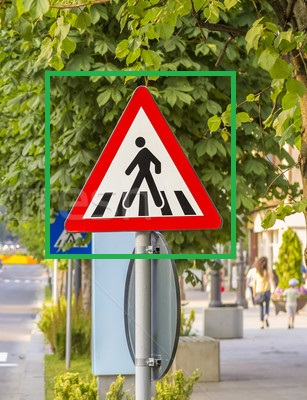
\includegraphics[width=4cm,height=4cm]{images/m06y4.jpg}
      \end{subfigure}
      \begin{subfigure}
      \centering
      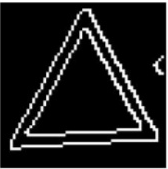
\includegraphics[width=4cm,height=4cm]{images/111.png}
      \end{subfigure}
    \caption{Exemple de seuillage de couleur rouge}
    \label{fig:seuillage de couleur}
\end{figure}

Alors que les chercheurs dans \cite{14} ont effectué la détection de couleur dans l'espace colorimétrique HSV (hue, saturation, value) et ils ont conclu que la saturation des couleurs varie considérablement lorsque les captures sont prises à partir de différents appareils. Certains d'autres \cite{15} ont étudié l'effet de la lumière sur la couleur des panneaux de signalisation pendant le jour et la nuit et ils ont conclu que la couleur de l'image pouvait être déformée par la lumière et que cela pouvait affecter la qualité des images (figure-\ref{fig:val rgb}).

\begin{figure}[h]
      \centering
    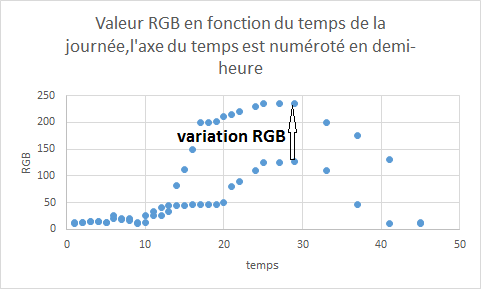
\includegraphics[width=8cm,height=4cm]{images/rgb.png}
    \caption{Valeur RGB en fonction du temps pour un pixel de signe STOP rouge \cite{15} }
    \label{fig:val rgb}
\end{figure}
{\textbf{Techniques basées sur des méthodes d'apprentissage de couleurs}}\\

Il existe plusieurs méthodes d'apprentissage de couleurs qui ont été mises en œuvre pour les panneaux de signalisation.\\
Les auteurs dans \cite{16} ont été les premiers, qui ont travaillé dans le domaine de l'algorithme génétique (GA) pour la détection de signes routiers, Ils ont détecté les panneaux de limitation de vitesse qui ont une forme ronde en utilisant un filtre de lissage et un filtre Laplacien pour éliminer le bruit, puis un algorithme génétique pour la détection de signes (figure-\ref{fig:GA}).\\

\begin{figure}[h]
      \centering
      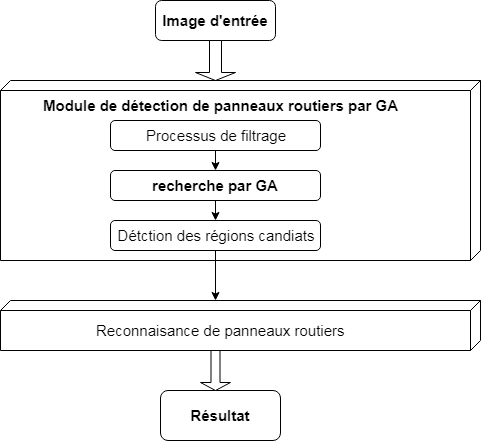
\includegraphics[width=10cm,height=7cm]{images/uu.png}
    \caption{Processus de détection en utilisant l'algorithme génitique (GA)\cite{16} }
    \label{fig:GA}
\end{figure}

Il y a aussi des algorithmes qui sont basés sur des machines à vecteurs de support (SVM),ce dernier a été proposé par les auteurs dans \cite{17} afin de classer les pixels en se référant sur les informations de couleurs, par contre Dans \cite{18}, les signes sont détectés à l'aide d'un ensemble de caractéristiques en ondelettes de Haar obtenues grâce à l'algorithme AdaBoost.\\
Les auteurs qui ont utilisé ces méthodes d’apprentissage de couleurs  ont conclu que cette dernière donne de meilleurs résultats par rapport à la segmentation par seuillage de couleur.
\subsection{ Détection basée sur la forme}

Les techniques de détection basées sur les couleurs ne sont utiles que si nous utilisons une caméra couleur de haute résolution et elle ne serait pas efficace dans toutes les conditions d’éclairage (la nuit ,les nuages…etc).\\
D’autre part,la détection peut aussi être faite par forme où il en existe plusieurs.\\

{\textbf{Détection de forme à l'aide des bords }}\\

Les techniques de détection de contour dépendent du contour des panneaux. Les auteurs dans \cite{19} ont effectué la détection de signes en utilisant un algorithme de correspondance de motifs rectangulaires simples.\\ 
Alors que d’autres comme par exemple \cite{20} ont utilisé l'équation d'ellipse pour détecter le cercle dans une image.
Cependant, la détection de forme à l'aide de fonctions périphériques ne peut donner des résultats précis que pendant la journée.\\

{\textbf{Détection de forme à l'aide d'une correspondance de modèle}}\\

Cette  méthode en général se base sur l’association entre l'image capturée et les  images de panneaux de signalisation routière de bonne qualité connus dans la base de données.\\ 
L’avantage principal de l’utilisation de cette méthode est qu’elle peut être modifiée pour détecter n’importe quel objet comme dans \cite{21} où « heldon.W et Oruklu » ont appliqué cette technique à l'appariement d'objets.\\

{\textbf{Détection basée sur des techniques d'apprentissage automatiques}}\\

Il y a diverses algorithmes qui peuvent être utilisés pour extraire la forme tels que les machines à vecteurs de support (SVM) et les réseaux de neurones (NN) qui sont les plus utilisés pour la détection de signes en raison de leurs capacité à détecter les formes avec précision.Cependant, concernant les réseaux de neurones, l’ajout de nouveau signes implique à nouveau la formation du réseau.\\ 
D’autres utilisent Les MSER (maximally stable extremal regions) comme dans \cite{21} qui fonctionnent sur les symboles de circulation avec un fond blanc dans laquelle les régions candidates sont détectées comme étant des régions extrêmes à stabilité maximale (MSER) ensuite les caractéristiques de l'histogramme des gradients orientés (HOG) sont dérivés.\\

{\textbf{Détection de forme basée sur la transformation de Hough (HT)}}\\

La transformation de "Hough" est utilisée pour détecter les cercles et les lignes sur la base d'un algorithme d'ajustement de courbes (Figure-\ref{fig:ht}).\\

Les auteurs dans \cite{22} se basent sur l'utilisation de la transformée de Hough standard afin de détecter la forme de la plaque de signalisation routière (par exemple circulaire, carrée, triangulaire,etc).
\begin{figure}[h]
      \centering
      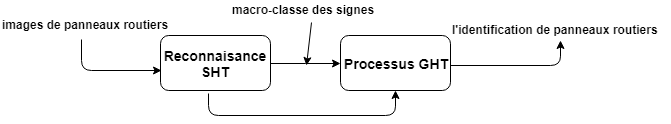
\includegraphics[width=16cm,height=4cm]{rt.png}
    \caption{Processus de détection proposé par \cite{22} en se basant sur Hough transform, SHT:Standard HT, GHT:Generalized HT.}
    \label{fig:ht}
\end{figure}

\section{Conclusion}

À partir de ce chapitre, on a eu une idée générale sur la phase de détection et ces techniques générales les plus utilisées, pour pouvoir constater l'importance de cette étape incontournable par rapport a un système de reconnaissance, tout en parcourant quelques travaux réalisés dans ce contexte.

\chapter{Reconnaissance des panneaux de signalisation}
\minitoc
\section{Introduction}
Une fois la première partie du système de reconnaissance qui est la détection est vu dans le chapitre précédent, Cette partie va être consacrée à la phase de reconnaissance elle-même ( qui est justement notre intérêt de travail), et les techniques utilisées pour réaliser un tel système tout en parcourant quelques travaux connexes concernant cette dernière.

\section{Reconnaissance des panneaux de signalisation}

Le résultat de l’étape de détection est une liste d’objets candidats qui pourraient être des panneaux de signalisation probables. Cette liste est transmise au dispositif de reconnaissance pour une évaluation ultérieure ensuite une classification afin de décider si les objets de la liste sont des objets rejetés ou des panneaux de signalisation en plus de leurs classes de décision.

\subsection{Caractéristiques d’un bon dispositif de reconnaissance }

Pour concevoir un bon système de reconnaissance, de nombreux paramètres doivent être pris en compte.

\begin{enumerate}
\item Le dispositif de reconnaissance doit présenter un bon pouvoir discriminant et un faible coût de calcul;
\item Il doit être robuste à l’état géométrique du signe, tel que l’orientation, la taille et la position du signe dans l’image;
\item Il doit être robuste au bruit;
\item La reconnaissance devrait être effectuée rapidement ;
\item Le classifieur doit pouvoir apprendre un grand nombre de classes d’où il vaut mieux utiliser autant que possible des connaissances a priori sur les panneaux de signalisation.
\end{enumerate}

\subsection{Défis du processus de la  reconnaissance des images}

D’un autre côté, il existe plusieurs défis qui opposent l’opération de la reconnaissance, une liste (non-exhaustive) de certaines difficultés est :
\begin{enumerate}
\item 
\begin{flushleft}
    
    Variation du point de vue\end{flushleft} Une seule instance d'un objet peut être orientée de plusieurs manières par rapport à la caméra(Figure-\ref{fig:variation});
    \begin{figure}[h]
      \centering
      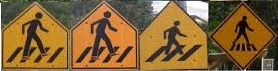
\includegraphics[width=12cm,height=3cm]{images.jpg}
    \caption{Exemple de variation de point de vue d'un panneau routier.}
    \label{fig:variation}
\end{figure}
 \pagebreak   
\item \begin{flushleft} Variation d'échelle\end{flushleft} Les classes visuelles présentent souvent des variations de tailles (Figure-\ref{fig:variation echel}) ;
 \begin{figure}[h!]
      \centering
      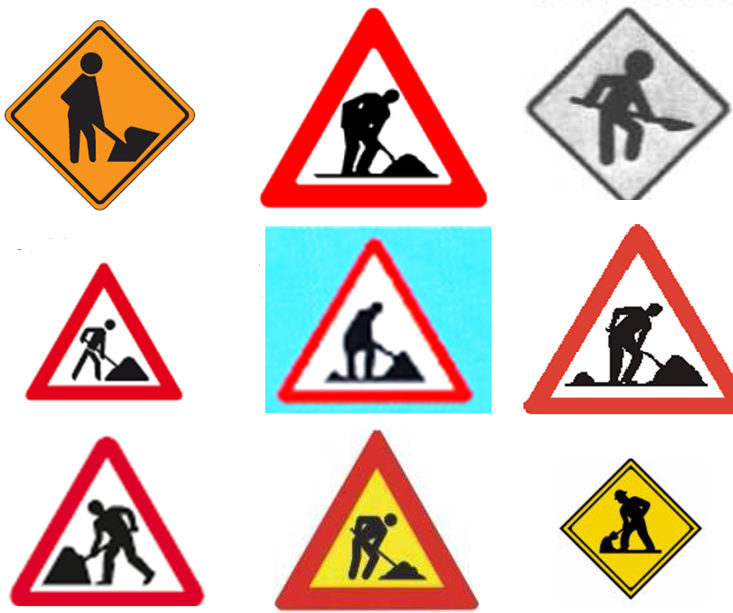
\includegraphics[width=10cm,height=4cm]{scale.png}
    \caption{Exemple de variation d'échelle pour un panneau routier représentant "travaux en cours".}
    \label{fig:variation echel}
\end{figure}
\item \begin{flushleft} Déformation\end{flushleft} De nombreux objets d'intérêt ne sont pas des corps rigides ou avec le facteur de l’âge peuvent être déformés de manière extrême (Figure-\ref{fig:deform});
\begin{figure}[h!]
      \centering
      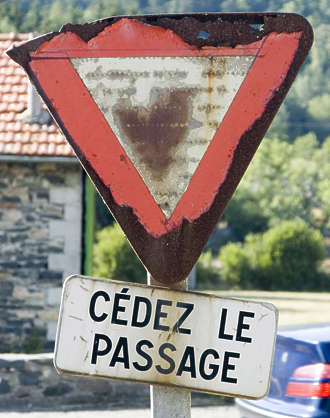
\includegraphics[width=5cm,height=3cm]{defo.jpg}
    \caption{Exemple de déformation d'un panneau routier}
    \label{fig:deform}
\end{figure}
\item \begin{flushleft} Occlusion\end{flushleft} Les objets d'intérêt peuvent être occultés. Parfois, seule une petite partie d'un objet peut être visible (Figure-\ref{fig:occlusion});
\begin{figure}[h]
      \centering
      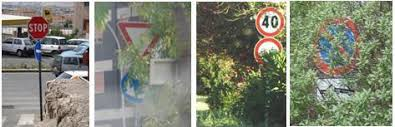
\includegraphics[width=14cm,height=4cm]{im.jpg}
    \caption{Exemple de panneaux routiers occultés.}
    \label{fig:occlusion}
\end{figure}
\newpage
\item  \begin{flushleft} Conditions d'éclairage\end{flushleft}Les effets de l'illumination ont une grande influence au niveau des pixels (Figure-\ref{fig:conditions});
\begin{figure}[h]
      \centering
      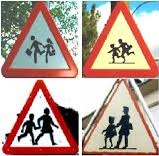
\includegraphics[width=8cm,height=4cm]{ec.jpg}
    \caption{Exemple d'effets d'éclairage sur un panneau routier.}
    \label{fig:conditions}
\end{figure}
\item \begin{flushleft} Fond désordonné\end{flushleft} Les objets d'intérêt peuvent se fondre dans leur environnement, ce qui les rend difficiles à identifier(Figure-\ref{fig:fond});
\begin{figure}[h!]
      \centering
      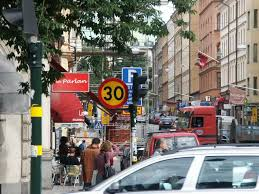
\includegraphics[width=8cm,height=5cm]{img.jpg}
    \caption{Exemple d'un fond désordonné.}
    \label{fig:fond}
\end{figure}
\pagebreak
\item  \begin{flushleft} Variation intra-classe \end{flushleft}
Les classes d'intérêt peuvent souvent être relativement larges, telles qu’il existe de nombreux types différents de ces objets, chacun ayant sa propre apparence (Figure \ref{fig:intraclasse}) .

\begin{figure}[h!]
      \centering
      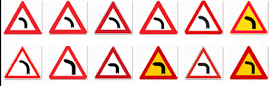
\includegraphics[width=8cm,height=4cm]{tl.png}
    \caption{Exemple de variation de plaques dans la même classe.}
    \label{fig:intraclasse}
\end{figure}
\end{enumerate}

Un bon système de reconnaissance des images doit être invariant pour le produit croisé de toutes ces variations,tout en conservant la sensibilité aux variations entre les classes.

\section{Méthodes de Reconnaissance }

Il existe plusieurs techniques utilisés pour la phase de reconnaissance dont on cite : K-plus proche voisin (K-nearest neighbor),Groupements de K-moyennes (K-mean clustering), Classifieur linéaire,Machines à vecteur de support(SVM) et les réseaux de neurones.

\subsection{Classifieur du voisin le plus proche (K-nearest neighbor) }

Ce classifieur prend une image test,et la compare à chacune des images d'apprentissage et prédit l'étiquette de l'image d'apprentissage la plus proche.\\
La notion de K-voisins plus proches présente une idée très simple: au lieu de trouver l'image la plus proche unique dans l'ensemble de formation, nous allons rechercher les k premières images les plus proches et les faire voter sur l'étiquette de l'image test. En particulier, lorsque k = 1, nous récupérons le classificateur  du voisin le plus proche.\\ Intuitivement, les valeurs élevées de k ont un effet de lissage qui rend le classifieur plus résistant aux valeurs éloignées.

\begin{figure}[h!]
      \centering
      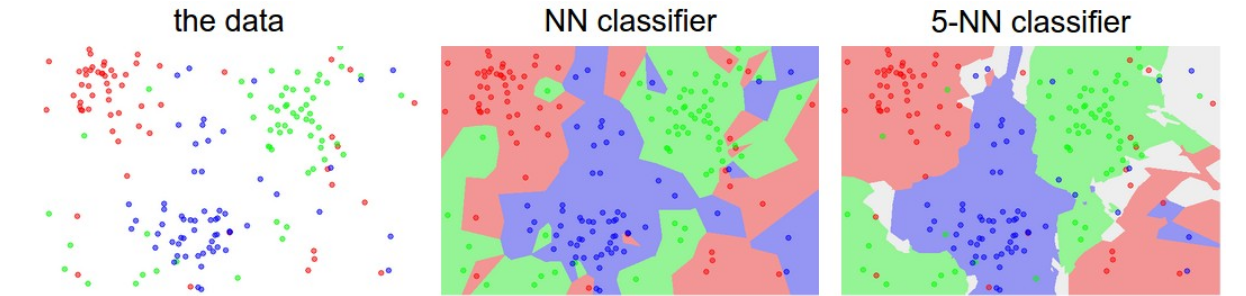
\includegraphics[width=15cm,height=5cm]{images/rgt.png}
    \caption{Exemple montrant la différence entre le classifieur de nearest neighbor(NN) et 5-nearest neighbor(5-NN),en utilisant des points à 2 dimensions et 3 classes (rouge, bleu, vert).}
    \label{fig:Knn}
\end{figure}
\newpage
Comme la Figure-\ref{fig:Knn} l'illustre,les régions colorées indiquent les limites de décision induites par le classifieur avec une distance « L ». Les régions blanches indiquent les points classés de manière ambiguë.Dans le cas d'un classifieur(NN), les points de données aberrants (par exemple, un point vert au milieu d'un nuage de points bleus) créent de petits îlots de prédictions probablement incorrectes, tandis que le classifieur 5-NN atténue ces irrégularités, ce qui entraîne probablement une meilleure généralisation.\\
D’après ce principe, on trouve que l’idée est simple du k-NN, mais le problème est quelle valeur de "K" il faut choisir et quel type de la distance il faut utilisé (distance de Manhattan, distance euclidienne, distance de Minkowski, distance de Tchebychev...etc).\\
Ces facteurs sont appelés des hyper-paramètres. La bonne façon de définir ces hyper-paramètres est de scinder les données d’entraînement en deux parties :

\begin{itemize}
    \item un ensemble d’entraînement et ;
    \item un ensemble de validation.
\end{itemize}

Ensuite il faut essayer différentes valeurs d'hyper-paramètres et conserver les valeurs qui permettent d'obtenir les meilleures performances sur l'ensemble de validation.\\
Il convient de prendre en compte certains avantages et inconvénients du classifieur du plus proche voisin.\\
De toute évidence, l’un des avantages est qu’il est très simple à mettre en œuvre et à comprendre. En outre, le classifieur ne prend pas de temps à s’entraîner, puisqu’il suffit de stocker les données d’entraînement. Cependant, nous payons ce coût de calcul au moment du test, car la classification d'un exemple de test nécessite une comparaison avec chaque exemple de formation. \\
De plus il y a plusieurs algorithmes et librairies qui peuvent accélérer la recherche du K-NN (exemple :{\textbf{ "FLANN"}} ).\\

Le classifieur du plus proche voisin peut, dans certains cas, être un bon choix dans certains paramètres (en particulier si les données sont de faible dimension), mais il est rarement approprié de l'utiliser pour la classification d'images pratiques. L’un des problèmes est que les images sont des objets de grande dimension et que les distances sur des espaces de grande dimension peuvent être très contre-intuitives.\\ 
Enfin, on peut dire que l’utilisation de distances sur des valeurs de pixels brutes n’est pas adéquate car les distances étaient davantage corrélées aux fonds d’arrière-plan et aux distributions de couleur des images qu’à leur contenu sémantique (Figure-\ref{fig:20}).
\begin{figure}[h!]
      \centering
      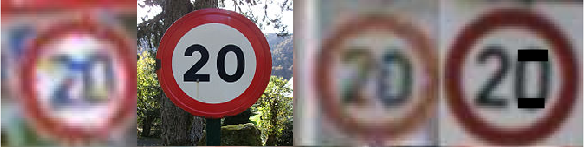
\includegraphics[width=15cm,height=4cm]{28.png}
      \caption{Exemple de résultat du classificateur K-NN, qui pour une image originale et trois autres images à côté de celle-ci, toutes à égale distance (la distance en pixels ne correspond pas du tout à une similarité perceptuelle ou sémantique).}
    \label{fig:20}
\end{figure}

D’autres parts, dans la littérature, les travaux concernant ce classifieur ne concerne pas la classification des images mais d’autres domaines,tel que \cite{25} dont les auteurs ont travaillé sur la connectivité du graphe pour la mise en cluster et la détection de valeurs aberrantes et dans \cite{26} une autre approche est présentée,qui utilise le K-NN pour classer le comportement des programme comme normal ou intrusif afin de détecter les intrusions et le comportement des programmes,...etc et bien plusieurs autres travaux.

\subsection{Le partitionnement en k-moyennes (K-means Clustering)}

La classification K-moyenne est un type d'apprentissage non supervisé, qui est utilisé dans le cas de données non étiquetées (c-à-d des données sans catégories ni groupes définis). Le but de cet algorithme est de trouver des groupes dans les données(Figure-\ref{fig:tt}), avec le nombre de groupes représentés par la variable K. L’algorithme fonctionne de manière itérative pour affecter chaque point de données à l’un des K groupes en fonction des caractéristiques fournies. Les points de données sont regroupés en fonction de la similarité des fonctionnalités \cite{27}.\\

\begin{figure}[h!]
      \centering
      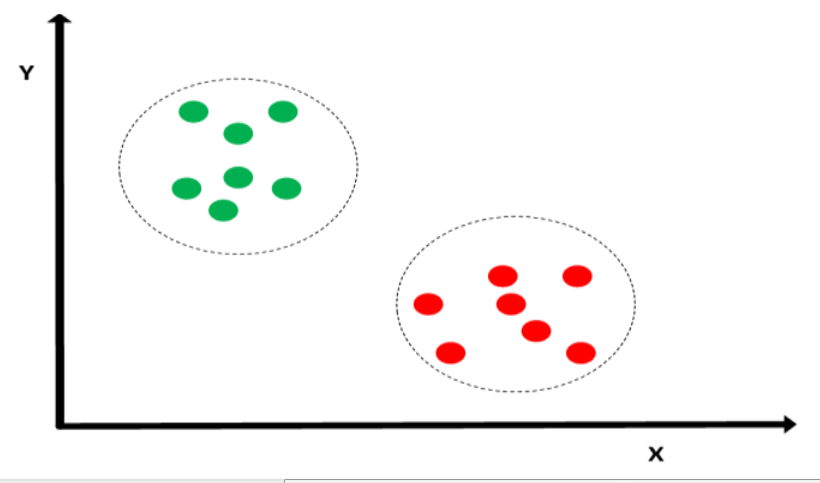
\includegraphics[width=10cm,height=4cm]{ttt.PNG}
      
    \caption{Exemple de groupes de clusters}
    \label{fig:tt}
\end{figure}
\newpage
Les résultats de l'algorithme de regroupement des k-moyennes sont :
\begin{itemize}
    \item Les centroïdes des groupes(centre de gravité des groupes );
    \item  Étiquettes pour les données d'apprentissage (chaque point de données est attribué à un seul cluster).
\end{itemize}
A part la détermination de groupes avant d'examiner les données, la mise en cluster permet de rechercher et d'analyser les groupes formés de manière organique. Le seul problème qui se pose lors de l’utilisation de ce genre d’algorithmes est le choix de K (nombre de groupes) qui sera détaillé prochainement dans ce qui suit.

\begin{enumerate}

\item L’algorithme de cette méthode \cite{28} est le suivant:\\ 

Les entrées de l'algorithme sont le nombre de groupes et l'ensemble de données. L'ensemble de données est un ensemble de caractéristiques pour chaque point de données.\\
L’algorithme commence par les estimations initiales pour les 'Κ' centroïdes, qui peuvent être générés de manière aléatoire.\\ 
L'algorithme itère ensuite entre deux étapes:

\begin{itemize}
    \item Étape d’affectation des données\\
Chaque centroïde définit l'un des groupes.Dans cette étape, chaque point de données est affecté à son centroïde le plus proche, en fonction de la distance euclidienne au carré. Plus formellement, si  "$c_i$" est la collection de centroïdes de l’ensemble C, chaque point de données x est affecté à un cluster en fonction de la formule suivante :
\[\underset{c_i \in C}{argmin \; dist\left (c_i,x\right )^2}\] 
\item Étape de mise à jour du centroïdes\\
Dans cette étape, les centres de gravités sont recalculés. Ceci est fait en prenant la moyenne de tous les points de données assignés au cluster de ce centre de gravité (formule ci-dessous):\\

\[ \ c_i=\frac{1}{|S_i|}\sum{x_i \in S_i x_i }\]
\end{itemize}
L'algorithme effectue une itération entre les étapes un et deux jusqu'à ce qu'un critère d'arrêt soit satisfait (c'est-à-dire qu'aucun point de données ne change pas de groupes, que la somme des distances est minimisée ou qu'un nombre maximal d'itérations est atteint).\\
Cet algorithme est garanti pour converger vers un résultat mais ce dernier peut être un optimum local et pas nécessairement le meilleur résultat possible.

\item Le choix de "k"\\ 
L'algorithme trouve les groupes et les étiquettes de jeu de données pour un "K" particulier pré-choisi.Pour trouver le nombre de groupes dans les données, l'utilisateur doit exécuter l'algorithme de classification K-moyenne pour une plage de K valeurs et comparer les résultats.\\
En général, il n'y a pas de méthode pour déterminer la valeur exacte de K, mais une estimation précise peut être obtenue en utilisant les techniques suivantes :
\begin{itemize}
\item La distance moyenne entre les points de données et leurs centre de gravité de groupes (centroïdes).Quand La distance moyenne au centroïde en fonction de K est tracée,le "point du coude", où le taux de diminution se déplace brusquement, peut être utilisé pour déterminer grossièrement K (Figure-\ref{fig:21}).
    
\begin{figure}[h!]
      \centering
      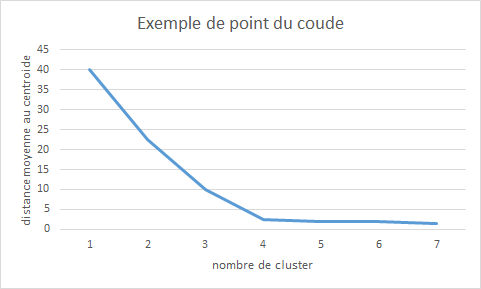
\includegraphics[width=12cm,height=5cm]{images/graph.png}
    \caption{Exemple montrant le point de coude}
    \label{fig:21}
\end{figure}
\item La validation croisée, 
\item Les critères d'informations,
\item La méthode de saut théorique,
\item La méthode de silhouette et l'algorithme de G-moyenne…etc.
\end{itemize}
\end{enumerate}

Au final, la surveillance de la répartition des points de données entre les groupes permet de mieux comprendre comment l’algorithme divise les données pour chaque K.\\

Il y a plusieurs travaux qui ont été réalisé dans le domaine de reconnaissance de panneaux de signalisations en utilisant les algorithmes de partitionnement en k-moyennes tel que \cite{29} qui porte sur l'application de la reconnaissance des conditions de conduite à la commande intelligente de véhicules électriques hybrides.À cette fin, les fonctions motrices sont identifiées et utilisées pour la mise en groupes, à l’aide de l’algorithme de mise en cluster en k-moyennes.

\subsection{Classifieur linéaire}
 
 Comme nous l’avons vu précédemment que le k-NN présente un certain nombre d'inconvénients:
 \begin{itemize}
     \item Le classifieur doit mémoriser toutes les données d'apprentissage et les stocker pour des comparaisons futures avec les données de test. C'est peu efficace en termes d'espace car les jeux de données peuvent facilement avoir une taille de 'gigaoctets'.
    \item Classer une image test est coûteux car cela nécessite une comparaison avec toutes les images d'apprentissage.
\end{itemize}

Alors que le classifieur linéaire présente une approche plus poussée pour la classification des images qui comporte deux composantes principales: une fonction de score (avec ses propres paramètres)qui mappe les données brutes aux scores de classe et une fonction de perte qui quantifiera l'accord entre les scores prédits et les étiquettes de vérité;
\begin{enumerate}
    \item Fonction de score \\
    La première étape de cette approche est de définir une fonction de score qui mappe les valeurs de pixels d'une image sur les scores de confiance de chaque classe. L’application linéaire utilisée est très simple :\\
          \[f(x_i,W,b)=Wx_i+b\] où :
\begin{itemize}
    \item Xi: présente la donnée d’apprentissage d’images chacune associée à une étiquette Yi et i=1...N exemples, j=1......K catégories distinctes ;
   \item W: matrice de poids ;
    \item b : vecteur de biais.
\end{itemize}
 
La Figure- \ref{fig:map} présente un exemple de mappage d’une image aux scores de classes où les pixels sont étendues en une colonne,après multiplication de matrices, on obtient les scores de chaque classe.

\begin{figure}[h!]
      \centering
      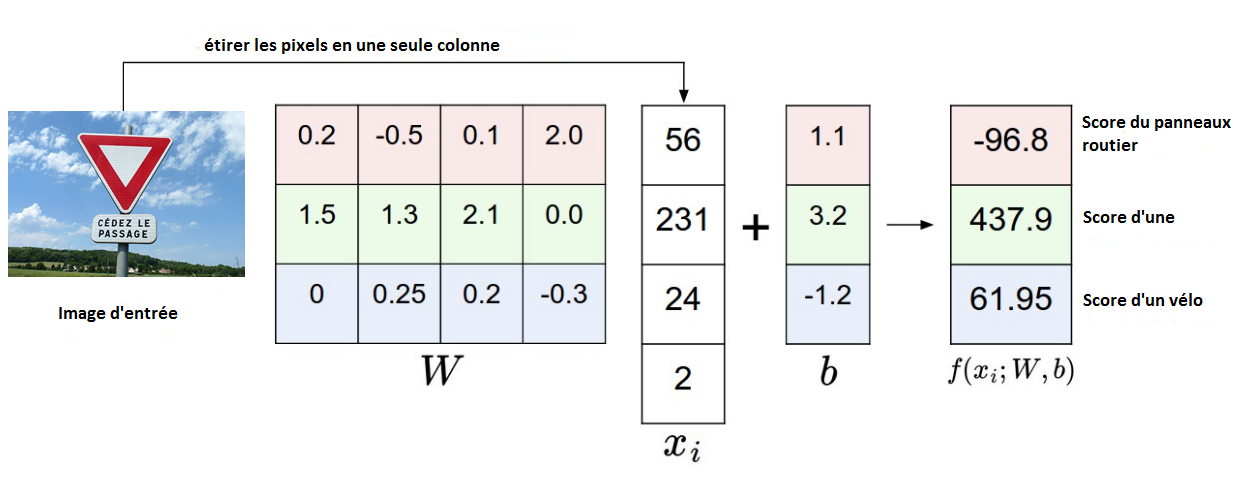
\includegraphics[width=14cm,height=5cm]{images/pp2.png}
    \caption{Exemple de mappage d’une image aux scores de classes}
    \label{fig:map}
\end{figure}
\newpage
\item Fonction de perte\\
Elle consiste à la mesure de la mécontente avec les résultats du classifieur, appelée aussi fonction de coût ou objective.\\

Principalement la perte sera importante si le classement des données de formation est mal fait et faible dans le cas contraire.Il existe plusieurs pertes mais les plus utilisés sont celles du « Softmax »et du « SVM » (les machines à vecteurs de support multi-classes).\\

Contrairement au classifieur « KNN »,l’avantage de cette approche paramétrique est qu’une fois que nous avons appris les paramètres (W,b) ,on peut par la suite ignorer les données d’apprentissage.\\
Il y a plusieurs recherches qui ont utilisé ce principe dans plusieurs problèmes liés au circulation des routes et aux panneaux de signalisation routière comme dans \cite{30} où les auteurs ont travaillé sur l’extraction de caractéristiques liées aux incidents des modèles de trafic.\\

La classification linéaire pour les vecteurs d'entrés bidimensionnels trace l'interprétation de la classification linéaire pour les vecteurs de suggestion bidimensionnels (Figure- \ref{fig:trc}) d’où l'espace est divisé en deux parties par les lignes en gras appelées « hyperplan » \cite{31}.
\end{enumerate}

\begin{figure}[h!]
      \centering
      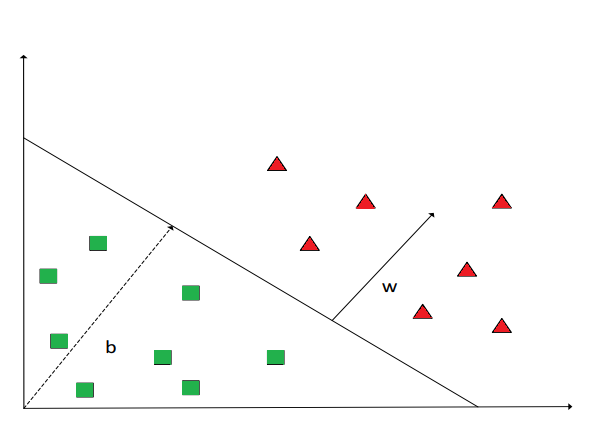
\includegraphics[width=8cm,height=5cm]{images/capt.png}
    \caption{Classification linéaire pour les vecteurs de suggestion}
    \label{fig:trc}
\end{figure}
\newpage
\subsection{Machines à vecteurs de support (SVM) }

Les machines à vecteurs de support (SVM) sont une classe d’algorithmes d'apprentissage supervisé destinées à résoudre des problèmes de discrimination (une technique statistique qui vise à décrire, expliquer et prédire l’appartenance à des groupes prédéfinis  d’un ensemble d’observations à partir d’une série de variables prédictives )et de régression qui a été proposée par « VAPNIK » en 1992 \cite{32}.\\

Les SVM sont une généralisation des classifieurs linéaires. Il utilise un espace d'hypothèses de fonctions linéaires, puis effectue la reconnaissance de formes en définissant des limites de décision qui séparent de manière optimale les données en catégories dans l'espace d'hypothèses.\\
Le principe du SVM est d’analyser et de trouver un hyperplan optimal tel que l’erreur de classification attendue pour les échantillons de test soit minimisée (Figure- \ref{fig:prin}).
\begin{figure}[h!]
      \centering
      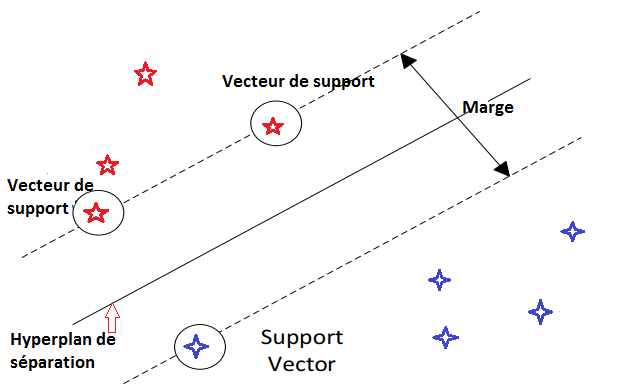
\includegraphics[width=8cm,height=5cm]{images/capt2.png}
    \caption{Principe de SVM}
    \label{fig:prin}
\end{figure}

Il existe des travaux différents qui entament cette approche dans le domaine de reconnaissance de panneaux de signalisation routière, on trouve dans \cite{33} un modèle de classification qui se base sur la forme en utilisant les machine à vecteurs de support et dans \cite{34} l’article traite le développement d’un ensemble de tests complet qui inclut toutes sortes de signes, il se base sur des machines à vecteurs de support pour la classification dont les motifs générés par les vecteurs représentent les distances aux frontières (DtB) des objets candidats à la signalisation.

\subsection{Réseaux de neurones artificiels (ANN)}

Les réseaux de neurones artificiels (Figure- \ref{fig:cc})ou « feed-forward neural network » introduits par \cite{35},sont un assemblage de neurones interconnectés les uns aux autres. L'objectif est de trouver une architecture qui produise la sortie souhaitée en fonction des entrées. Les principaux paramètres sont la "forme" du réseau et les poids des différentes liaisons \cite{36}.

\begin{figure}[h!]
      \centering
      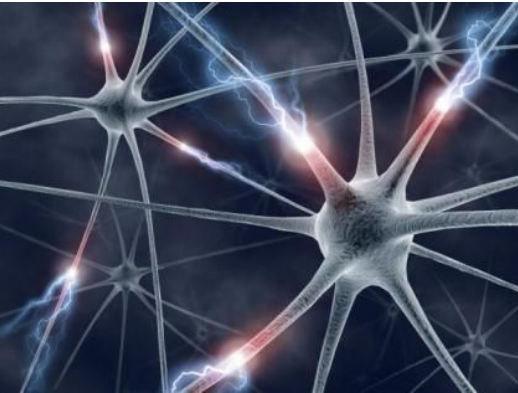
\includegraphics[width=5cm,height=3cm]{images/neurone.png}
    \caption{Réseau de neurones}
    \label{fig:cc}
\end{figure}

{\textbf{Paradigme biologique}}\\

Les neurones sont des cellules nerveuses qui constituent l’unité fondamentale de base pour le système nerveux. Ils ont le rôle de faire circuler les informations en externe (entre l'environnement et l'organisme) et en interne (au sein de l'organisme) de plus de leurs excitabilités c'est-à-dire la capacité de répondre aux stimulations et de convertir celles-ci en impulsions nerveuses.\\
\newpage
{\textbf{Structure des neurones} }

\begin{figure}[h!]
      \centering
      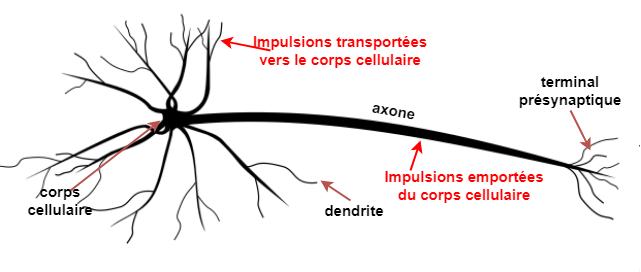
\includegraphics[width=10cm,height=5cm]{images/neurone2.png}
    \caption{Composition d'un neurone}
    \label{fig:compp}
\end{figure}

Un neurone est composé de (Figure-\ref{fig:compp} ):
\begin{enumerate}
    \item D’un corps cellulaire qui comporte le le noyau ;
\item Des dendritiques (ou prolongements) qui reçoivent les signaux en provenance d’autres cellules ;
\item D’un axone par où sont diffusées les informations.
\end{enumerate}
Les axones et les dendritiques de neurones entrent en contact et transmettent l'information de cellule à cellule via des structures spécialisées : les synapses.\\
Les neurones sont au nombre de 100 milliards dans le cerveau humain et sont donc capables de créer un réseau très complexe, avec parfois plus de 100.000 synapses par neurone.\\

{\textbf{Réseaux de neurones artificiels }}\\

Le traitement automatique de l’information cherche à s’évolué du jour à l’autre,d’où la nouvelle approche qui se base sur l’inspiration du fonctionnement effectuée par le  cerveau humain dont le comportement intelligent est sous-tendu par un ensemble de mécanismes mentaux. Ces mécanismes sont principalement basés sur des processus neurophysiologiques et c’est depuis ces hypothèses que les réseaux de neurones artificiels se sont développés.\\ 
Chaque neurone artificiel est un processeur élémentaire. Il reçoit un nombre variable d'entrées en provenance de neurones amonts.\\

A chacune de ces entrées est associée un poids « W » qui représente de la force de la connexion. Chaque processeur élémentaire est doté d'une sortie unique, qui se ramifie ensuite pour alimenter un nombre variable de neurones .Ce modèle de neurone est appelé neurone formel (Figure- \ref{fig:mod}).

\begin{figure}[h!]
      \centering
      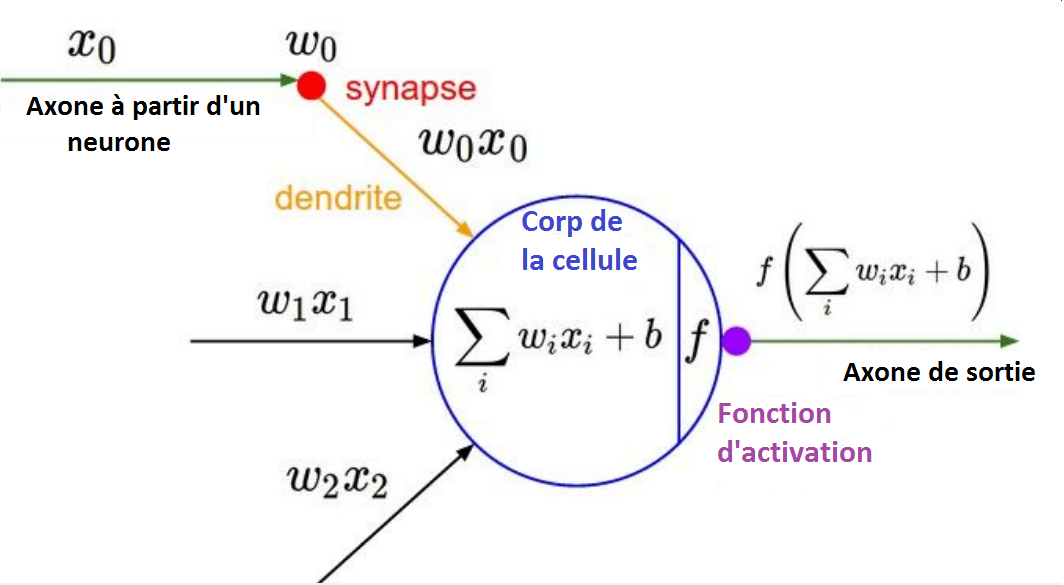
\includegraphics[width=10cm,height=8cm]{images/model.png}
    \caption{Modéle d'un réseau de neurones}
    \label{fig:mod}
\end{figure}

Un neurone formel a comme entrées  X1,X2,....Xn, f une fonction d’activation, la sortie est: \[f(\sum w_i x_i + b)\] où la fonction d’activation opère une transformation d’une combinaison affine des signaux d’entrée, et l’utilisation d’une constante qui est le biais du neurone « b ».\\
Dans un réseau de neurones artificiels, on distingue trois types de neurones \cite{37}:
\begin{itemize}
    \item Les neurones d’entrées, aussi appelés cellules perceptives car ils captent des données dont la provenance est en dehors du réseau;
    \item Les neurones de sortie, qui définissent la sortie du réseau;
    \item Les neurones cachés, qui n’ont aucune relation avec le monde extérieur au réseau mais juste avec les autres neurones du réseau. 
    
\end{itemize}

Les différents types de neurones se distinguent par la nature de leurs fonction d’activation f, et les principaux types sont:

\begin{itemize}
    \item Linéaire :   f est la fonction identité;
    \item Sigmoïde : \[f(x)=1/(1+e^{x})\] 
    \item Rectified linear unit (ReLU): \[f(x)=max(0;x)\] 
\end{itemize}
\newpage
{\textbf{Apprentissage}}\\

L'apprentissage est la propriété la plus intéressante des réseaux neuronaux. C’est une phase du développement d'un réseau de neurones durant laquelle le comportement du réseau est modifié jusqu'à l'obtention du comportement désiré \cite{38}.\\
Il présente la modification des poids du réseau dans le but d'accorder la réponse du réseau aux exemples et à l'expérience. Il est souvent impossible de décider à priori des valeurs des poids d'un réseau pour une application donnée, à l'issu de l'apprentissage, les poids seront fixés.\\
Selon les algorithmes d'apprentissage, il a été défini deux grandes classes :l'apprentissage supervisé ou non supervisé. Cette distinction repose sur la forme des exemples d'apprentissage. Dans le cas de l'apprentissage supervisé, les exemples sont des couples (Entrée, Sortie associée) alors que l'on ne dispose que des valeurs (Entrée) pour l'apprentissage non supervisé. Cependant que les modèles à apprentissage non supervisé nécessitent avant la phase d'utilisation une étape de labélisation, qui n'est pas autre chose qu'une part de supervision.\\

{\textbf{Perceptron multicouche}}\\

Les perceptrons multicouches sont parmi les topologies les plus utilisé qui décrivent les connexions dans un réseau.\\
Les perceptrons multicouches (PMC) ou Multi-Layer Perceptron (MLP) est un type de réseau de neurone qui impose que les neurones soient organisés en couches successives, ou chacune est entièrement connectée à la couche suivante et précédente (Figure- \ref{fig:couche}) \cite{48}.

\begin{figure}[h!]
      \centering
      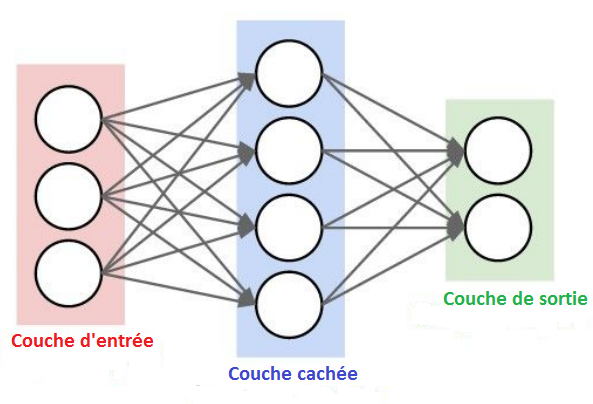
\includegraphics[width=9cm,height=6cm]{images/moddl.png}
    \caption{Exemple de couche cachée}
    \label{fig:couche}
\end{figure}
\newpage
{\textbf{Travaux liés}}\\

Il y a plusieurs travaux qui se sont basés sur les réseaux de neurones avec leurs différents types pour la reconnaissance de panneaux de signalisation routière, on trouve  dans \cite{39} l’utilisation de  réseaux de neurones profonds pour la reconnaissance à partir du référentiel allemand de reconnaissance des panneaux de signalisation (GTSRB) qui a remporté la phase finale de ce dernier en 2012 où il était le seule à avoir obtenu un taux de reconnaissance supérieur à l'être humain de 99,46 percent ou dans \cite{40} où une architecture neuronale profonde (CNN «convolutional neural network» et RBFNN « radial basis function neural network») est mise en œuvre pour effectuer la classification des panneaux de signalisation afin d'améliorer le taux de reconnaissance des panneaux de signalisation. Il y a aussi les auteurs de \cite{41} qui se sont basé sur les réseaux de neurones artificiels basiques pour la classification, ainsi que \cite{42} où la reconnaissance est basée sur un réseau de neurones à plusieurs couches de perceptrons.\\
\section {Étude Comparative}
On se basant sur les recherches effectuées dans la littérature, une étude comparative concernant les techniques précédemment citées pour la reconnaissance des panneaux de signalisation révèle une importance primordiale pour notre travail afin de pouvoir se positionner par rapport à ses différentes techniques.\\

Dans \cite{43,44}, une étude comparative a été effectuée concernant les méthodes de classification permettant d’identifier les panneaux de signalisation .Ces méthodes de classification sont le réseau neuronal artificiel (ANN), les k-voisins les plus proches (kNN), la machine à vecteurs de support (SVM).Donc, Une base de données publique bien connue sera utilisée pour des fins de comparaison qui est GTRSB (German Traffic Sign Recognition database), qui a montré que les réseaux de neurones artificiels donnent la précision la plus faible de 76 pourcent,   et le taux d'erreur le plus élevé comme montré dans le tableau si dessous.\\ 

En revanche, KNN réalise la performance la plus élevée avec une précision de 92 pourcent comme indiqué dans le (Tableau- \ref{table:res}) bien que KNN soit le meilleur classifieur parmi d’autres, le processus de classification prend beaucoup de temps.Par conséquent, pour une mise en œuvre en temps réel il est déconseillé de l’utiliser.\\
\newpage
\begin{table}[]
\centering
\begin{tabular}{|l|l|l|}
\hline
\multicolumn{1}{|c|}{Classifieur} & \multicolumn{1}{c|}{ Précision (\%)} & \multicolumn{1}{c|}{taux d'erreur(\%)} \\ \hline
\multicolumn{1}{|c|}{ANN}    & \multicolumn{1}{c|}{76.8667 }  & \multicolumn{1}{c|}{23.1333}\\ \hline
\multicolumn{1}{|c|}{KNN (K=1)}    & \multicolumn{1}{c|}{92.333}  & \multicolumn{1}{c|}{7.6566}\\ \hline
\multicolumn{1}{|c|}{SVM}    & \multicolumn{1}{c|}{&86.2666}  & \multicolumn{1}{c|}{4.3566}\\ \hline
\end{tabular}
\caption{Résultats de comparaison entre les méthodes de reconnaisances: K-NN,SVM,ANN \cite{43,44}}
\label{table:res}
\end{table}

Selon \cite{43}, la meilleure approche adaptée pour la reconnaissance des images est le KNN ,mais compte tenu des point négatifs vu précédemment dans la partie concernant ce modèle, il est pas conseiller de confier une reconnaissance des images au classifieur KNN .\\

D’un autre coté \cite{40} montre une étude comparative concernant deux types de réseaux de neurones très utlisés pour la classification des images :
\begin{itemize}
    \item CNN ou «convolutional neural network» : c’est un type de réseau neuronal d'architecture profonde;
    \item RBFNN ou « radial basis function neural network »: c’est un type de réseau neuronal d’architecture réseau de neurones d’architecture peu profonde.
\end{itemize}

 Par conséquent, les résultats expérimentaux dans \cite{40} ont montré qu'un réseau de neurones à architecture profonde offre de meilleures performances qu'un réseau de neurones à architecture peu profonde(Tableau- \ref{table:reess}) ,d’où les auteurs de ce travail conseillent fortement l’utilisation des CNN pour la reconnaissance des images.\\
 \begin{table}[]
\centering
\begin{tabular}{|l|l|l|}
\hline
\multicolumn{1}{|c|}{Classifieur} & \multicolumn{1}{c|}{ Précision (\%)} & \multicolumn{1}{c|}{taux d'erreur(\%)} \\ \hline
\multicolumn{1}{|c|}{RBFNN}    & \multicolumn{1}{c|}{40 }  & \multicolumn{1}{c|}{90}\\ \hline
 \multicolumn{1}{|c|}{CNN}    & \multicolumn{1}{c|}{99}  & \multicolumn{1}{c|}{2}\\ \hline
\end{tabular}
\\captionof{Résultats de comparaison entre les méthodes de reconnaisances: RBFNN,CN \cite{40}}
\label{table:reess}
\end{table}
 
\section{Méthode de reconnaissance adaptée pour ce travail}
D’un côté, vu que la classification des images repose sur des tâches de reconnaissance visuelle, les récents développements en matière de réseaux de neurones (Deep Learning) ont considérablement amélioré les performances de ces systèmes de reconnaissance visuelle à la pointe de la technologie. Et d’un autre coté vu que les résultats obtenues montrent que l’utilisation de réseaux de neurones à architecture profonde (CNN) donne un résultat de 99 pourcent du taux de reconnaissance des panneaux de signalisation et un taux d’erreur inférieur à celui donné par tous les classifieurs étudiés.\\

De plus, que notre intérêt porte sur le domaine du « Deep Learning »,notre approche de reconnaissance de panneaux de signalisation adaptée dans ce travail, va être basée sur les réseaux de neurones à convolution(CNN), et ce dernier va être détaillé dans le chapitre suivant.


\section{Conclusion}
Le but de ce chapitre était de faire une vue d’ensemble sur le processus de reconnaissance et surtout souligner les techniques les plus utilisés dans ce processus tout en parcourant les travaux et les recherches réalisés à propos de ces techniques et finir par une étude comparative afin d’avoir une décision raisonnable par rapport à la technique qui va être adoptée dans ce travail pour la reconnaissance de panneaux de signalisation routière tout en se référant de  recherches et d’expérience effectuées dans la littérature  .



